

This chapter starts with a description of basic concepts of molecular biology (Section~\ref{sec:basic.concepts.molecular.biology}). This section is oriented towards readers who are not familiarized with biological sciences and will be based generally in Alberts et al.~\cite{alberts2007} and Lodish et al.~\cite{lodish2007}. Next, our biological narrative narrows towards the principles of eukaryotic regulation (Section~\ref{sec:eukaryotic.regulation}), which will be based on Alberts et al.~\cite{alberts2007}, Lodish et al.~\cite{lodish2007}, Maston et al.~\cite{maston2006} and Allis et al.~\cite{allis2007} (Section~\ref{sec:chromatin.epigenetics}). This discussion includes all the necessary terms for the understanding of the problem addressed in this work. Next, the problem of active transcription factor binding site detection is introduced (Section~\ref{sec:active.binding.site.detection}). In this section we will: (1) define the problem, (2) show how it is traditionally addressed by computational methods, (3) introduce the novel biological experiments based on next-generation sequencing and (4) discuss how the problem is currently being addressed using computational frameworks and the novel biological experiments. Also, in this section we will discuss the challenges associated to the problem of active binding site detection and our approach to address these challenges, which were not considered by previous methods. Next, we provide a comprehensive literature review on the prediction of transcription factor binding sites using next-generation sequencing data within computational frameworks (Section~\ref{sec:literature.review}). 


#########################


%%%%%%%%%%%%%%%

In the rest of this section we will characterize the aforementioned types of \emph{cis}-acting regulatory regions.


%%%%%%%%%%%%%%%%%%%%%%%%%%%%%%%%%%%%%%%%%%%%%%%%%%%%%%%%%%%%%%%%%%%%%
% Subsection: Promoter Core
%%%%%%%%%%%%%%%%%%%%%%%%%%%%%%%%%%%%%%%%%%%%%%%%%%%%%%%%%%%%%%%%%%%%%
\subsection{Promoter Core}
\label{sec:promoter.core}

% Promoter core introduction
The promoter core is the region where the elements from the general transcriptional machinery binds to start the transcription. First, the general transcription factors -- which includes the RNA polymerase and many auxiliary proteins -- assemble at this region forming the pre-initiation complex (PIC), which directs the RNA polymerase to the transcription start site (TSS). Then, the transcription is ready to undergo the elongation phase.

% Promoter core elements
There are many well-studied binding units within the promoter core such as the initiator element (Inr), the TATA box, the downstream core element (DCE), the TFIIB-recognition element (BRE) and the motif ten element (MTE). All these transcription factor binding sites interact with general transcription factors (mostly, the TFIID) to start the PIC assembly.

%%%%%%%%%%%%%%%%%%%%%%%%%%%%%%%%%%%%%%%%%%%%%%%%%%%%%%%%%%%%%%%%%%%%%
% Subsection: Proximal Regulatory Elements
%%%%%%%%%%%%%%%%%%%%%%%%%%%%%%%%%%%%%%%%%%%%%%%%%%%%%%%%%%%%%%%%%%%%%
\subsection{Proximal Regulatory Elements}
\label{sec:proximal.regulatory.elements}

% Proximal promoter elements
The proximal promoter elements are located immediately upstream the promoter core. This region is composed of several transcription factor binding sites which may enhance (through the binding of activator proteins) or decrease (through the binding of repressor proteins) the expression of a gene, upon binding of particular transcription factors. Approximately $60\%$ of proximal regulatory elements (within promoters) are located next to CpG islands, which are DNA regions composed of a high number of C and G nucleotides and a higher frequency of CpG dinucleotides (i.e. a C followed by a G in the same strand). The difference of nucleotide frequencies between regulatory regions \emph{versus} non-regulatory regions is now evident and will be further explored in this work.

% Activators. re[ressprs and co-binding
It is also very common for activator and repressor TFs to bind together with other proteins. This phenomenon is called co-binding. Furthermore, we call co-activator and co-repressor, TFs that generally bind with activators and repressors, respectively. It is known that co-binding processes have a synergistic characteristic, i.e. the real effect of the co-bound partners is higher than the expected summation of their effects when binding separated.

%%%%%%%%%%%%%%%%%%%%%%%%%%%%%%%%%%%%%%%%%%%%%%%%%%%%%%%%%%%%%%%%%%%%%
% Subsection: Enhancers
%%%%%%%%%%%%%%%%%%%%%%%%%%%%%%%%%%%%%%%%%%%%%%%%%%%%%%%%%%%%%%%%%%%%%
\subsection{Enhancers}
\label{sec:enhancers}

% Enhancers
Enhancer elements regulate the temporal and spatial expression of a gene and do not depend on the distance from the promoter regions (which can be up to \approxy$1,000,000$ bp) or on its orientation with regard to the promoters. This region is typically composed by several transcription factor binding sites close to each other, where specific proteins bind to enhance the expression of a target gene. The TFs that bind to the enhancer regions are called activators. Furthermore, the expression of a specific gene can be modulated by different enhancers in different cell conditions, in response to different stimuli. Moreover, the spatial organization and orientation of the TFBSs composing the enhancer region can be vital for its regulatory activity.

% DNA looping
Enhancers are similar in function to the proximal activator elements and the difference between their mechanism is still under investigation. In fact, many TFs that bind to proximal regions also bind to enhancer regions. The current model on how these distal enhancer regions activate the gene is based on DNA looping. In this model, the DNA conforms in such a way that, although the enhancer is several base pairs away from the gene being regulated, it gets physically close to the promoter core and is able to act on the structures assembled at this proximal region. Recent research even suggests that some PIC factors assemble at enhancer regions and through DNA looping it aggregates to the rest of the general TFs in order to start transcription. Nevertheless, it is expected that novel experimental assays that enables us to visualize the three-dimensional DNA conformation elucidates the mechanisms in which distal regions interact with promoter proximal elements.

%%%%%%%%%%%%%%%%%%%%%%%%%%%%%%%%%%%%%%%%%%%%%%%%%%%%%%%%%%%%%%%%%%%%%
% Subsection: Silencers
%%%%%%%%%%%%%%%%%%%%%%%%%%%%%%%%%%%%%%%%%%%%%%%%%%%%%%%%%%%%%%%%%%%%%
\subsection{Silencers}
\label{sec:silencers}

% Silencers
Silencers are regions that contains TFBSs in which proteins bind to decrease the expression of a gene. The TFs that bind to the silencer regions are called repressors. Similarly to enhancer regions, the silencer activity does not depend on the distance to the promoter region of the gene being regulated nor the orientation between the silencer and the proximal region. However, some silencers which depend on the position (in reference to the promoter of the regulated gene) were found. The complexity arises with the fact that silencer regions can be found not only as a separate independent regions (like most enhancers), but also: (1) within enhancer regions -- adding further regulatory complexity to its mechanism and (2) in relatively proximal regions. Further complexity is added given the fact that some activator TFs can change their expression enhancing capabilities into a strong repressive effect via the binding with some particular co-factors.  

% Silencer mechanism
The silencers can repress the expression in many ways: (1) not allowing the binding of an essential activator TF or a general component of the transription machinery, physically blocking their binding or directly competing for the same TFBS; (2) inhibiting the formation of the PIC at the promoter core and (3) recruiting special proteins that modifies the DNA structure in such a way that does not allow the binding of activator TFs to proximal regulatory elements or disables the binding of the own main transcriptional machinery at the promoter core.

%%%%%%%%%%%%%%%%%%%%%%%%%%%%%%%%%%%%%%%%%%%%%%%%%%%%%%%%%%%%%%%%%%%%%
% Subsection: Insulators
%%%%%%%%%%%%%%%%%%%%%%%%%%%%%%%%%%%%%%%%%%%%%%%%%%%%%%%%%%%%%%%%%%%%%
\subsection{Insulators}
\label{sec:insulators}

% Insulators
Insulator regions, also known as boundary elements, block the action of other regulatory elements by ``partitioning'' the genome in blocks, in which each block has its own internal regulatory mechanisms. They are bound by TFs with high molecular weight and long binding residence time. This disables some regulatory regions at one side of the insulator to act on genes or other regulatory regions at the other side. The insulators have two specific properties and known modes of action: (1) block the influence of an enhancer over the expression of a particular gene by disabling the communication between the enhancer and the gene's promoter region and (2) block the spread of gene silencing that occurs via proteins that change the DNA structure (which usually work as a chain reaction, stopping at insulator regions). Therefore, insulator elements are position-dependent, however their orientation does not seem to be important.

% CTCF
Although a number of TFs that bind to insulator regions are known for organisms such as \emph{Drosophila}, in vertebrates, only one TF is known -- the CTCF (CCCTC-binding factor). The binding of this TF in insulator regions can be regulated in several ways, including DNA methylation, post-translational modifications and interaction with co-factors.

%%%%%%%%%%%%%%%%%%%%%%%%%%%%%%%%%%%%%%%%%%%%%%%%%%%%%%%%%%%%%%%%%%%%%
% Subsection: Locus Control Regions
%%%%%%%%%%%%%%%%%%%%%%%%%%%%%%%%%%%%%%%%%%%%%%%%%%%%%%%%%%%%%%%%%%%%%
\subsection{Locus Control Regions}
\label{sec:locus.control.regions}

% Locus control regions
Locus control regions (LCRs) are groups of regulatory elements such as enhancers, silencers and insulators, all of which are involved in the regulatory mechanism of an entire locus, i.e. genomic region consisting of a group of a number of genes. These regions are operationally defined as elements that drive the tissue-specific physiological expression in a form that is independent of its position and dependent on the number of copy number variations (CNVs). The TFs that bind these regions (activators, co-activators, repressors, co-repressors or DNA shape modifiers) affect the expression of genes in different ways and its their collective activity that confers the specific function of each LCR.





########################






%%%%%%%%%%%%%%%%%%%%%%%%%%%%%%%%%%%%%%%%%%%%%%%%%%%%%%%%%%%%%%%%%%%%%
% Subsection: DNase I Footprinting
%%%%%%%%%%%%%%%%%%%%%%%%%%%%%%%%%%%%%%%%%%%%%%%%%%%%%%%%%%%%%%%%%%%%%
\subsection{DNase I Footprinting}
\label{sec:dnase.i.footprinting}

% DNase I Digestion
The DNase I footprinting method consists in the observation of the DNA digestion by a certain cleavage agent able to break the phosphodiester bonds of the DNA molecule. The cleavage agent used in this method is the endonuclease deoxyribonuclease I (DNase I). This enzyme is capable of binding at the DNA double helix's minor groove and break the phosphodiester bond. This enzyme is of particular interest to this experiment design because of its great size, which makes it sensitive to proteins bound on DNA. Also, the action of DNase I can be easily controlled with ethylenediaminetetraacetic acid (EDTA).

% Method explanation - extraction, PCR and eletrophoresis
The method initiates with the retrieval of genomic DNA. Given the genomic DNA of multiple cells, the region of interest is amplified via polymerase chain reaction (PCR). The amplification step generates many DNA molecules identical to the original, which needs to be between 50--200 bp. After amplification, the resulting fragments are labeled with fluorescent molecules and are separated in two sets. In one set the protein of interest is added to bind the DNA and in the other set is reserved (without protein) as a control set. Then, DNase I is added in both sets, which will cut the fragments at random locations. Afterwards, an electrophoresis procedure is applied on both cleaved fragment sets. Finally, it is applied some agent that enables the visualization of the fluorescent marker.

% Method explanation - results
The distribution of the fragments will ressemble a ladder. The shorter DNA fragments are closer to the positive extremity of the electrophoresis tray and the longer DNA fragments are closer to the origin (negative extremity). Then, we must compare both DNA fragment sets (the one treated with protein and the control). Given the fact that the DNase I enzyme is not able to cleave the DNA in regions where there are proteins already bound to the DNA (because it is not able to access the region), fluorescent visualization of fragments with certain lengths will be visible in the control set but not in the protein-treated set. Therefore, the lack of lanes in the protein-treated electrophoresis' results indicates that there was a protein bound to that region. We call these regions footprints. The rationale of this method is depicted in Figure~\ref{fig:song_dnase_footprinting}.

% Conclusion
The advantage of this method is that it is spatially very precise on locating a protein binding site in the DNA. However, the DNase I footprinting method does not identify which protein was bound. Furthermore, this technique is complex to be executed and needs a considerable number of initial cells. Nevertheless, the main disadvantage of this method is that it is a low-throughput method, i.e. it is able to analyze only small portions of the genome in a single assay (few hundreds of base pairs).

% Figure - DNase I footprinting 
% TODO - Caption
\begin{figure}[h!]
\centering
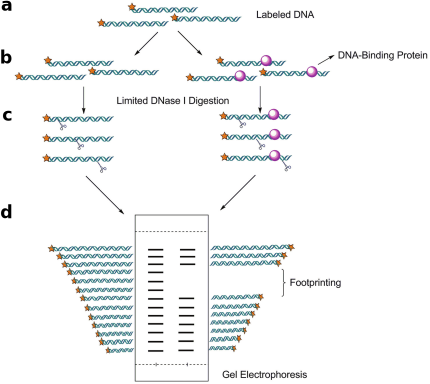
\includegraphics[width=0.6\textwidth]{song_7_dnase_footprinting}
\caption[DNase I footprinting]{\textbf{DNase I footprinting.} Placeholder. \emph{Source: Song et al.}\cite{song2015} (modified to fit thesis format and/or clarify key points).}
\label{fig:song_dnase_footprinting}
\end{figure}

%%%%%%%%%%%%%%%%%%%%%%%%%%%%%%%%%%%%%%%%%%%%%%%%%%%%%%%%%%%%%%%%%%%%%
% Subsection: Chromatin Immunoprecipitation
%%%%%%%%%%%%%%%%%%%%%%%%%%%%%%%%%%%%%%%%%%%%%%%%%%%%%%%%%%%%%%%%%%%%%
\subsection{Chromatin Immunoprecipitation}
\label{sec:chromatin.immunoprecipitation}

% ChIP
The chromatin immunoprecipitation (ChIP) consists in the observation of DNA regions enriched with a particular target protein. This technique can also be used to identify proteins with post-translational modifications, such as the methylated/acetylated histones. Furthermore, differently from DNase I footprinting, this technique is able to identify DNA-protein interactions \emph{in vivo}, i.e. the protein-DNA interactions are preserved from the source organism's cells, instead of induced using test tubes (\emph{in vitro}).

% Method explanation
Briefly, the ChIP works as follows. First, the cell's chromatin is accessed. Then, the DNA and associated proteins on the chromatin are crosslinked, i.e. the protein-DNA interactions are preserved with artificial covalent bonds. Afterwards the crosslinked chromatin is sheared into approximately $200$ bp DNA fragments with any massive shearing procedure (sonication, ultraviolet radiation or endonucleases). After shearing, the crosslinked DNA fragments associated with the target protein are selectively immunoprecipitated by using an antibody that can bind to the target protein. Then, the immunoprecipitated DNA$+$protein complexes are purified and the resulting DNA fragments are sequenced. Finally, we can determine the approximate location of the target protein's binding site by mapping the sequenced fragments into the organism's genome. The rationale of this method is depicted in Figure~\ref{fig:lodish_chip}.

% Conclusion
It is important to point the differences between DNase I footprinting and ChIP. As previously mentioned, in the DNase I footprinting method, we determine the binding of any protein in the region being analyzed, without knowing which protein is binding; however in the ChIP we only determine the binding of a particular target protein with a known antybody in the region of interest. Furthermore, while the DNase I footprinting gives the precise protein binding location, the ChIP tells us an approximated region for the binding of the target protein, since the protein can be virtually anywhere within the \approxy$200$ bp immunoprecipitated fragments. The selection of the technique to use depends mainly on the experimental design and should consider these important details. However, as in the DNase I footprinting technique, ChIP is also low-throughput. Therefore, we are only able to analyze a very small portion of the genome at each experiment.

% Figure - Chromatin immunoprecipitation
% TODO - Caption
\begin{figure}[h!]
\centering
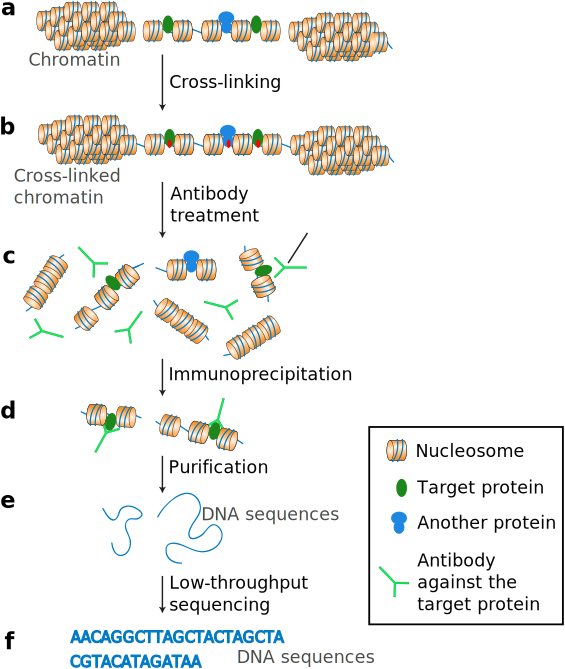
\includegraphics[width=0.6\textwidth]{lodish_487_chip}
\caption[Chromatin immunoprecipitation]{\textbf{Chromatin immunoprecipitation.} Placeholder. \emph{Source: Lodish et al.}\cite{lodish2007} (modified to fit thesis format and/or clarify key points).}
\label{fig:lodish_chip}
\end{figure}




############################




%%%%%%%%%%%%%%%%%%%%%%%%%%%%%%%%%%%%%%%%%%%%%%%%%%%%%%%%%%%%%%%%%%%%%
% Subsection: Eukaryotic Regulation Overview
%%%%%%%%%%%%%%%%%%%%%%%%%%%%%%%%%%%%%%%%%%%%%%%%%%%%%%%%%%%%%%%%%%%%%
\subsection{Eukaryotic Regulation Overview}
\label{sec:eukaryotic.regulation.overview}

% Conclusion on regulatory overview
The previous discussion represented a brief depiction on eukaryotic regulation. We presented the main terms that are necessary for the understanding of this work. We summarize here some key points:

\begin{itemize}
  \item Proteins called transcription factors (TFs) bind to regions in the DNA called transcription factor binding sites (TFBSs).
  \item Regulatory regions, which generally contain multiple TFBSs, can appear next to the gene being regulated (such as the promoter region) or several base pairs up-- or downstream (such as enhancers).
  \item Features that remodel chromatin structure also play very important roles in the regulation of gene expression. One of the most-studied features is the post-translational histone tail modification.
\end{itemize}

% Conslusion on regulatory overview
However, gene regulation is an active field of study. Novel mechanisms are discovered frequently and build up to shape our understanding of the bigger picture. The Figure~\ref{gusmao_overview_regulation} summarizes the concepts reviewed so far in a single framework.

% TODO [MAYBE] Figure: The bigger picture of regulation: This picture containing the cell nucleus, cell signaling, chromosome regions, chromatin conformation, histone modifications, transcription factor binding and the DNA level.
\begin{figure}[h!]
\centering
\includegraphics[width=0.5\textwidth]{gusmao_overview_regulation}
\caption[Overview of the eukaryotic regulatory features]{\textbf{Overview of the eukaryotic regulatory features.} Placeholder.}
\label{fig:gusmao_overview_regulation}
\end{figure}




######################



%%%%%%%%%%%%%%%%%%%%%%%%%%%%%%%%%%%%%%%%%%%%%%%%%%%%%%%%%%%%%%%%%%%%%
% Section: Chromatin Structure and Epigenetics
%%%%%%%%%%%%%%%%%%%%%%%%%%%%%%%%%%%%%%%%%%%%%%%%%%%%%%%%%%%%%%%%%%%%%
\section{Chromatin Structure and Epigenetics}
\label{sec:chromatin.epigenetics}

In the previous section we discussed the main features of eukaryotic regulation at the level of transcription initiation and the elements behind the regulatory processes. In this section we will situate the eukaryotic regulation processes within the chromatin dynamics context. The term chromatin is used to define the complex of macromolecules found in the cell nucleus consisting of DNA, protein and RNA. First, we will discuss the chromatin structure. Then, we will introduce the term epigenetics and discuss the epigenetic elements necessary for the understanding of this work. Finally, we will finish this section with an overview of the bigger picture regarding eukaryotic regulation and all its complexities.

%%%%%%%%%%%%%%%%%%%%%%%%%%%%%%%%%%%%%%%%%%%%%%%%%%%%%%%%%%%%%%%%%%%%%
% Subsection: Chromatin Structure
%%%%%%%%%%%%%%%%%%%%%%%%%%%%%%%%%%%%%%%%%%%%%%%%%%%%%%%%%%%%%%%%%%%%%
\subsection{Chromatin Structure}
\label{sec:chromatin.structure}

% Chromatin structure 1
The DNA is not isolated in the cell nucleus. Instead, the DNA conforms in many organizational levels. The DNA is found wrapped in a set of eight proteins called histone complex, which are generally composed of four pairs of the histones named H2A, H2B, H3 and H4. The unit composed by the DNA wrapped in approximately $1.65$ turns (\approxy$147$ bp) around the histone complex is called nucleosome. From this lower level structure (nucleosome) the chromatin structure can be compacted in many different levels. This compaction organization is depicted in Figure~\ref{fig:lodish_chromatin_structure}. Briefly, the chromatin can be found in a very condensed structure which does not allow transcription initiation (termed heterochromatin, or simply ``closed chromatin''); or in a decondensed form, allowing transcription initiation and gene expression (termed euchromatin, or simply ``open chromatin'').

% Figure - Chromatin conformation
% TODO - Caption
\begin{figure}[h!]
\centering

\includegraphics[width=0.4\textwidth]{lodish_420_chromatin_structure}
\caption[Chromatin conformation]{\textbf{Chromatin conformation.} Placeholder. \emph{Source: Lodish et al.}\cite{lodish2007} (modified to fit thesis format and/or clarify key points).}
\label{fig:lodish_chromatin_structure}
\end{figure}

% Chromatin structure 2
Different parts of the genome can be open and closed at different times, allowing a specific set of genes to be expressed under different cell conditions. This is one of the main mechanisms in which we are able to observe such a high number of different cells, each of which expressing a different set of genes, given that they all share the same underlying genomic information encoded in the DNA. The Figure~\ref{fig:lodish_open_closed_chromatin} shows a graphical example of two cells at different stages of commitment. Although the genomic region (locus) depicted is the same for these two cells, one present a closed chromatin structure, while the other present an open chromatin structure. The closed chromatin observed for the long-term hepatopoietic stem cell (Figure~\ref{fig:lodish_open_closed_chromatin}a) does not allow the gene ATF3 to be transcribed, while the open chromatin structure present in the monocyte cell (Figure~\ref{fig:lodish_open_closed_chromatin}b) does allow the expression of ATF3 gene, since the transcription factors and transcription machinery are able to access that region and start the transcription process.

% Chromatin remodelling mechanisms
The chromatin can switch between closed and open states via two major chromatin remodelling mechanisms: (1) covalent post-transcriptional histone modifications by specific enzymes such as histone acetyltransferases (HATs), deacetylases, methyltransferases and kinases and (2) ATP-dependent chromatin remodelling complexes which either move, eject or restructure nucleosomes. In Figure~\ref{fig:lodish_open_closed_chromatin}, we depict some post-transcriptional histone modifications which are indicative of open/closed chromatin regions. In the next subsection we will discuss the post-transcriptional histone modifications in detail.

% Figure - Open versus closed chromatin
% TODO - Caption
\begin{figure}[h!]
\centering
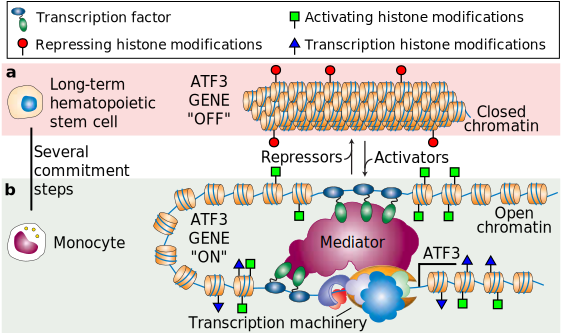
\includegraphics[width=0.9\textwidth]{lodish_461_open_closed_chromatin}
\caption[Open \emph{versus} closed chromatin]{\textbf{Open \emph{versus} closed chromatin.} Placeholder. \emph{Source: Lodish et al.}\cite{lodish2007} (modified to fit thesis format and/or clarify key points).}
\label{fig:lodish_open_closed_chromatin}
\end{figure}

%%%%%%%%%%%%%%%%%%%%%%%%%%%%%%%%%%%%%%%%%%%%%%%%%%%%%%%%%%%%%%%%%%%%%
% Subsection: Epigenetics and Histone Modifications
%%%%%%%%%%%%%%%%%%%%%%%%%%%%%%%%%%%%%%%%%%%%%%%%%%%%%%%%%%%%%%%%%%%%%
\subsection{Epigenetics and Histone Modifications}
\label{sec:epigenetics.histone.modifications}

% Epigenetic features
Epigenetics can be briefly defined as the study of the variations within gene expression and consequent phenotypic traits which are caused by other features than the information contained in the DNA. i.e. functional genomic changes that do not involve changes in DNA. There are a number of well-studied epigenetic mechanisms that also regulates the expression of genes, such as: (1) Post-translational modifications of certain amino acids in histones; (2) chromatin remodelling through ATP-dependent processes that changes the position of nucleosomes; (3) insertion or removal of histone variants into the chromatin structure; (4) small non-coding RNAs and (5) DNA methylation. Thereafter, we will focus on the first feature of the aforementioned list.

% Histone modifications
The histone proteins n-terminal usually protrudes from the nucleosome and is termed histone tail. These histone tails can undergo post-translational chemical modifications at specific amino acids. These modifications include the methylation (addition of a methyl group), acetylation (addition of an acetyl group), phosphorylation (addition of a phosphoryl group), ubiquitylation (addition of a ubiquitin protein) and sumoylation (addition of SUMOs -- small ubiquitin-like modifiers). These modifications have a specific nomenclature dictated by: histone type, amino acid type, amino acid position within the histone tail and modification type. For instance, ``H3K4me1'' refers to the monomethylation (me1) of the fourth lysine (K4) of the tail of histone H3.

% Histone modification effects on chromatin
The histone modifications are directly associated to regulatory events since they change the accessibility of proteins to the DNA in the chromatin, enabling or disabling the binding of TFs (see Figure~\ref{fig:lodish_open_closed_chromatin}). For instance, the HATs are able to transfer an acetyl group to certain amino groups of histone tail's lysine side chains. In doing so, they neutralize the lysine's positive charge and makes the interactions between histones and DNA weaker. Consequently, the DNA is more accessible for TF binding. The Figure~\ref{fig:lall_histone_modifications} displays most known histone modification effects on chromatin structure.

% TODO - Caption
\begin{figure}[h!]
\centering
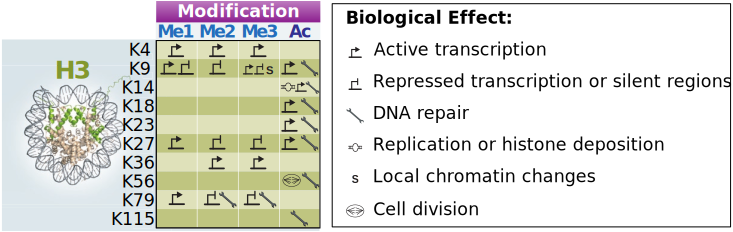
\includegraphics[width=0.7\textwidth]{lall_1111_histone_modifications}
\caption[Main histone modifications on lysines of histone H3]{\textbf{Main histone modifications on lysines of histone H3.} Placeholder. \emph{Source: Lall et al.}\cite{lall2007} (modified to fit thesis format and/or clarify key points).}
\label{fig:lall_histone_modifications}
\end{figure}





##############


% Introduction on NGS - recap
In Section~\ref{sec:dnase.i.footprinting} and Section~\ref{sec:chromatin.immunoprecipitation} we discussed two experimental methods to detect active transcription factor binding site. However, these methods are able to analyze only a small part of the genome at a given assay. Therefore, it is virtually impossible to perform a genome-wide analysis using such low-throughput methods.




##################





